\documentclass[12pt]{article}

% =========================
% Packages
% =========================
\usepackage[margin=1in]{geometry}
\usepackage{setspace}
\usepackage{booktabs}
\usepackage{longtable}
\usepackage{array}
\usepackage{amsmath}
\usepackage{amssymb}
\usepackage{amsthm}
\usepackage{hyperref}
\usepackage{tikz}
\usetikzlibrary{positioning,arrows.meta}

\hypersetup{
  colorlinks=true,
  linkcolor=black,
  urlcolor=blue,
  citecolor=black
}

\setlength{\parskip}{0.6em}
\setlength{\parindent}{0pt}
\onehalfspacing

% =========================
% Theorem Environments
% =========================
\newtheorem{definition}{Definition}
\newtheorem{axiom}{Axiom}
\newtheorem{proposition}{Proposition}
\newtheorem{lemma}{Lemma}
\newtheorem{remark}{Remark}

% =========================
% Document
% =========================
\begin{document}

\begin{center}
{\LARGE \textbf{The Dickinson Climate Classification}}\\
\vspace{0.25em}
{\large Caleb Dickinson}
\end{center}

% ============================================================
\section*{Abstract}

We introduce the Dickinson Climate Classification, a thermodynamically grounded, species-independent framework for classifying past, present, future, and hypothetical climates. The system explicitly separates thermal constraints from hydrological constraints, restricts aridity classification to climates that are neither polar, subpolar, or alpine, and defines all classification boundaries using evenly spaced physical thresholds. Importantly, the system does not attempt to define the absolute limits of life; instead, it partitions climate space into analytically useful categories for comparative and predictive analysis across Earth’s paleoclimates, present climates, projected future warming scenarios, and ecologically relevant climatic states that may never occur on Earth.

\section*{Relation to Existing Climate Classification Systems}

The Dickinson Climate Classification differs fundamentally in purpose and
structure from widely used systems such as Köppen and UNEP.
The Köppen system is explicitly ecological and biogeographic, with
classification thresholds calibrated to the present-day distribution of
vegetation and climatic analogues on Earth.
The UNEP aridity index, by contrast, is development-oriented, designed
primarily to assess land degradation and desertification risk rather than
to partition climate space as a whole.
In contrast, the Dickinson classification is formulated as a thermodynamic
state-space partition, independent of biological distributions and
socioeconomic objectives.
This distinction permits consistent classification across paleoclimates,
future warming scenarios, and ecologically relevant climatic states that
may never be realized on Earth, without requiring revision of thresholds
or category definitions.

% ============================================================
\section{Foundational Principles}

\begin{axiom}[Earth as a Subset of Hypothetical Climate Space]
Let $\mathcal{C}$ denote the set of all hypothetical climate regimes in which life is physically possible.  
The set of all Earth climates constitutes a proper subset of $\mathcal{C}$.
\end{axiom}

\begin{remark}
This axiom does not assert that all partitions of climate space defined by this system can be realized on Earth, but instead establishes a formal climate state space within which Earth’s climates may be situated, compared, and extended under paleoclimatic and future boundary conditions.
\end{remark}

\begin{axiom}[Species Independence]
Classification thresholds shall not be defined using the present-day
distribution limits of biological taxa.
The climatic tolerances of all species shift over evolutionary time,
as lineages diverge from common ancestors and adapt to changing
environmental conditions.
\end{axiom}

\begin{axiom}[Dimensionless Aridity Partitioning]
All aridity regimes in the Dickinson classification are defined exclusively
by dimensionless ratios of hydrological quantities.
No aridity boundary is specified using absolute precipitation totals,
absolute evapotranspiration totals, or fixed millimeter thresholds.
Consequently, aridity classification is invariant under uniform rescaling
of hydrological fluxes and depends only on relative water balance.
\end{axiom}

\begin{axiom}[Partition, Not Habitability]
The Dickinson classification partitions continuous climate space into analytically useful regions but does not define the absolute bounds of life.  
Climates or microclimates that differ substantially in biological extremity (e.g., hypothetical thermophile-dominated regimes in $55^\circ$C $T_{\max,\text{mean}}$ versus $80^\circ$C $T_{\max,\text{mean}}$) may be assigned to the same category if they occupy the same region of thermodynamic climate space.
\end{axiom}

\begin{remark}
This axiom ensures that the classification remains stable under evolutionary adaptation, paleoclimatic variability, and future warming scenarios, without requiring revision in response to newly discovered extremophiles or altered biological tolerances.
\end{remark}

\begin{axiom}[Domain of Applicability]
The Dickinson classification is defined only over the subset of climate space in which life is physically possible.  
Outside this domain, the classification is not meaningful and no interpretation is implied.
\end{axiom}

% ============================================================
\section{Thermal Definitions}

\begin{definition}[Climatological Monthly Means]
Let $T_m$ denote the climatological mean near-surface air temperature of month $m \in \{1,\dots,12\}$, averaged over a standard 30-year normal period.
\end{definition}

\begin{definition}[Coldest-Month Mean Temperature]
\[
T_{\min,\text{mean}} = \min_{m}(T_m)
\]
\end{definition}

\begin{definition}[Warmest-Month Mean Temperature]
\[
T_{\max,\text{mean}} = \max_{m}(T_m)
\]
\end{definition}

% ============================================================
\section{Part I: Cold-Month Thermal Zones}

\begin{definition}[Cold-Month Thermal Zone Assignment]
Given the climatological coldest-month mean temperature
$T_{\min,\text{mean}}$, the cold-month thermal zone
$\mathcal{T}_{\text{cold}}$ is defined by:
\[
\mathcal{T}_{\text{cold}} \in
\begin{cases}
\text{Hypercaneal (H)} & [50,\infty) \\
\text{Uninhabitable (X)} & [40,50) \\
\text{Hyperequatorial (Z)} & [30,40) \\
\text{Equatorial (A)} & [20,30) \\
\text{Tropical (B)} & [10,20) \\
\text{Subtropical (C)} & [0,10) \\
\text{Temperate (D)} & [-10,0) \\
\text{Continental (E)} & [-20,-10) \\
\text{Subarctic (F)} & [-30,-20) \\
\text{Arctic (G)} & [-40,-30) \\
\text{Superarctic (Y)} & (-\infty,-40)
\end{cases}
\quad \text{(°C)}
\]
\end{definition}

% ============================================================
\section{Part II: Aridity Relevance}

\begin{definition}[Aridity Relevance Condition]
Aridity classification applies if and only if:
\[
T_{\max,\text{mean}} \ge 15^\circ\text{C}
\quad \land \quad
T_{\min,\text{mean}} \ge -30^\circ\text{C}.
\]
\end{definition}

\begin{proposition}
If the aridity relevance condition is not satisfied, the moisture regime of the climate is undefined within the Dickinson system.
\end{proposition}

\begin{remark}
This excludes permafrost-dominated, polar, and cold-summer climates, where PET approaches zero and precipitation seasonality does not meaningfully structure ecosystems.
\end{remark}

% ============================================================
\section{Hydrological Definitions}

\begin{definition}[Annual Precipitation]
\[
P_{\text{ann}} = \sum_{m=1}^{12} P_m
\]
\end{definition}

\begin{definition}[Annual Potential Evapotranspiration]
\[
PET_{\text{ann}} = 12 \cdot PET_{\text{mean}}
\]
\end{definition}

\begin{definition}[Aridity Index]
\[
AI = \frac{P_{\text{ann}}}{PET_{\text{ann}}}
\]
\end{definition}

% ============================================================
\section{Part II: Aridity Regimes}

\begin{definition}[Baseline Aridity Regimes]
Given aridity relevance, a climate is assigned an aridity regime by:
\[
AI \in
\begin{cases}
(0.75,\infty) & \text{Humid (H)} \\
(0.50,0.75] & \text{Semihumid (G)} \\
(0.25,0.50] & \text{Semiarid (S)} \\
(0,0.25] & \text{Arid Desert (D)}
\end{cases}
\]

This is modified from the UNEP aridity index shown below:
\[
AI \in
\begin{cases}
(0.65,\infty) & \text{Humid} \\
(0.50,0.65] & \text{Dry subhumid} \\
(0.20,0.50] & \text{Semi-arid} \\
(0.05,0.20] & \text{Arid} \\
(0,0.05] & \text{Hyperarid}
\end{cases}
\]
\end{definition}

% ============================================================
\section{Seasonality Diagnostics}

\begin{definition}[High-Sun Precipitation Fraction]
Let $P_{\text{hs}}$ be precipitation during the six highest-insolation months:
\[
HS = \frac{P_{\text{hs}}}{P_{\text{ann}}}
\]
\end{definition}

\begin{definition}[Rolling Six-Month Dominance]
\[
P6 = \max_{k}\left(\sum_{j=0}^{5} P_{((k+j-1)\bmod 12)+1}\right),
\quad
P6ratio = \frac{P6}{P_{\text{ann}}}
\]
\end{definition}

% ============================================================
\section{Aridity Overrides}

\begin{definition}[Mediterranean Regime]
A climate is classified as Mediterranean (M) if:
\[
AI > 0.25 \;\land\;
\begin{cases}
HS < 0.4 & \text{Northern extratropics} \\
HS > 0.6 & \text{Southern extratropics}
\end{cases}
\]
\end{definition}

\begin{definition}[Monsoon Regime]
A climate is classified as Monsoon (W) if:
\[
P6ratio \ge 0.8,
\]
excluding climates already classified as Mediterranean or Arid Desert.
\end{definition}

\begin{definition}[Temperate Rainforest Override]
Let $P_{\text{driest}}$ be the minimum monthly precipitation.  
If a Mediterranean-classified climate satisfies:
\[
P_{\text{driest}} \ge \frac{PET_{\text{ann}}}{12 \cdot 20},
\]
then it is reclassified as Humid (H).
\end{definition}

\begin{remark}
The denominator $12 \cdot 20$ explicitly represents a threshold of 5\% of mean monthly PET, scaled to annual PET. This formulation avoids an opaque constant while preserving dimensional clarity.
\end{remark}

\begin{figure}[htp]
\centering
\resizebox{\textwidth}{!}{%
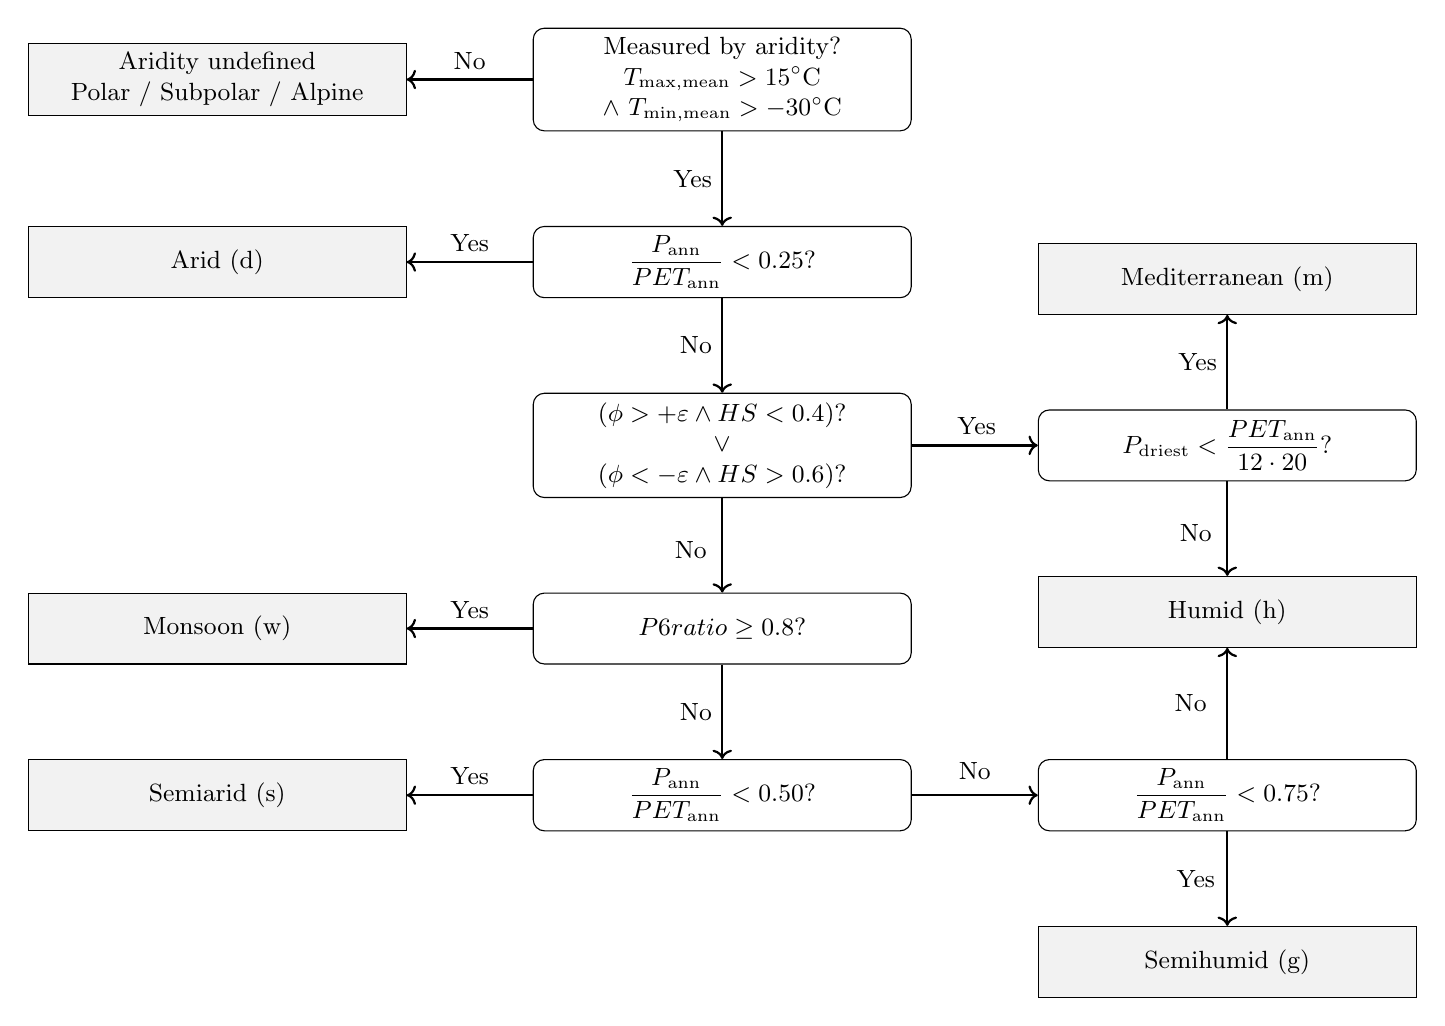
\begin{tikzpicture}[
  node distance=12mm and 16mm,
  decision/.style={
    rectangle, draw, rounded corners,
    align=center, font=\small,
    minimum width=4.8cm, minimum height=9mm
  },
  outcome/.style={
    rectangle, draw,
    align=center, font=\small,
    fill=gray!10,
    minimum width=4.8cm, minimum height=9mm
  },
  arrow/.style={->, thick}
]

% =====================================================
% START
% =====================================================

\node[decision] (relevance)
{Measured by aridity?\\
$T_{\max,\mathrm{mean}} > 15^\circ\mathrm{C}$\\
$\land\ T_{\min,\mathrm{mean}} > -30^\circ\mathrm{C}$};

\node[outcome, left=of relevance] (polar)
{Aridity undefined\\
Polar / Subpolar / Alpine};

\draw[arrow] (relevance) -- node[above,font=\small]{No} (polar);

% =====================================================
% ARID CHECK
% =====================================================

\node[decision, below=of relevance] (aridcheck)
{$\dfrac{P_{\mathrm{ann}}}{PET_{\mathrm{ann}}} < 0.25$?};

\node[outcome, left=of aridcheck] (arid)
{Arid (d)};

\draw[arrow] (relevance) -- node[left,font=\small]{Yes} (aridcheck);
\draw[arrow] (aridcheck) -- node[above,font=\small]{Yes} (arid);

% =====================================================
% MEDITERRANEAN CHECK
% =====================================================

\node[decision, below=of aridcheck] (medcheck)
{$(\phi > +\varepsilon \land HS < 0.4)?$\\
$\lor$\\
$(\phi < -\varepsilon \land HS > 0.6)?$};

\draw[arrow] (aridcheck) -- node[left,font=\small]{No} (medcheck);

\node[decision, right=of medcheck] (medoverride)
{$P_{\text{driest}} < \dfrac{PET_{\text{ann}}}{12 \cdot 20}$?};

\node[outcome, below=of medoverride] (humid)
{Humid (h)};

\node[outcome, above=of medoverride] (med)
{Mediterranean (m)};

\draw[arrow] (medcheck) -- node[left,font=\small, xshift=4mm, yshift=2.5mm]{Yes} (medoverride);
\draw[arrow] (medoverride) -- node[above,font=\small, xshift=-4mm, yshift=-3mm]{No} (humid);
\draw[arrow] (medoverride) -- node[left,font=\small]{Yes} (med);

% =====================================================
% MONSOON CHECK
% =====================================================

\node[decision, below=of medcheck] (monsooncheck)
{$P6ratio \ge 0.8$?};

\node[outcome, left=of monsooncheck] (monsoon)
{Monsoon (w)};

\draw[arrow] (medcheck) -- node[above,font=\small, xshift=-4mm, yshift=-3mm]{No} (monsooncheck);
\draw[arrow] (monsooncheck) -- node[above,font=\small]{Yes} (monsoon);

% =====================================================
% HUMIDITY SPLIT
% =====================================================

\node[decision, below=of monsooncheck] (semiaridcheck)
{$\dfrac{P_{\mathrm{ann}}}{PET_{\mathrm{ann}}} < 0.50$?};

\node[outcome, left=of semiaridcheck] (semiarid)
{Semiarid (s)};

\draw[arrow] (monsooncheck) -- node[left,font=\small]{No} (semiaridcheck);
\draw[arrow] (semiaridcheck) -- node[above,font=\small]{Yes} (semiarid);

\node[decision, right=of semiaridcheck] (semihumidcheck)
{$\dfrac{P_{\mathrm{ann}}}{PET_{\mathrm{ann}}} < 0.75$?};

\draw[arrow] (semiaridcheck) -- node[below,font=\small, yshift=5.5mm]{No} (semihumidcheck);

\node[outcome, below=of semihumidcheck] (semihumid)
{Semihumid (g)};

% NOTE: Humid (H) node already exists elsewhere
\draw[arrow] (semihumidcheck) -- node[above,font=\small, xshift=-4mm, yshift=-2.5mm]{Yes} (semihumid);
\draw[arrow] (semihumidcheck) -- node[right,font=\small, xshift=-8mm]{No} (humid);

\end{tikzpicture}
}

\caption{
Decision tree for assigning aridity regimes in the Dickinson
classification.\\\\
\textbf{Note:} $\phi$ denotes geographic latitude in degrees.
Mediterranean seasonality is evaluated only at extratropical locations,
defined as latitudes whose absolute value exceeds the Earth’s instantaneous
axial tilt (i.e., poleward of the tropics).
}
\end{figure}

% ============================================================
\section{Part III: Warm-Month Thermal Zones}

\begin{definition}[Warm-Month Thermal Zone Assignment]
Given the climatological warmest-month mean temperature
$T_{\max,\text{mean}}$, the warm-month thermal zone
$\mathcal{T}_{\text{warm}}$ is defined by:
\[
\mathcal{T}_{\text{warm}} \in
\begin{cases}
\text{Hypercaneal Summer (H)} & [50,\infty) \\
\text{Hyperthermal Summer (X)} & [40,50) \\
\text{Scorching Summer (z2)} & [35,40) \\
\text{Very Hot Summer (z1)} & [30,35) \\
\text{Hot Summer (a2)} & [25,30) \\
\text{Warm Summer (a1)} & [20,25) \\
\text{Cool Summer (b2)} & [15,20) \\
\text{Cold Summer (b1)} & [10,15) \\
\text{Very Cold Summer (c2)} & [5,10) \\
\text{Freezing Summer (c1)} & [0,5) \\
\text{Frigid Summer (Y)} & (-\infty,0)
\end{cases}
\quad \text{(°C)}
\]
\end{definition}

% ============================================================
\section{Illustrative Complete Climate Codes}

The following examples demonstrate the semantic interpretation of
complete Dickinson climate codes.  
Each code is composed of a cold-month thermal zone, an aridity regime
(where applicable), and a warm-month thermal zone, as defined in the
preceding sections.  
These examples are illustrative only and do not necessarily exist on earth.

\begin{itemize}
  \item \textbf{YY} —
  Superarctic with frigid summer (aridity classification undefined).

  \item \textbf{Fa2} —
  Subarctic with hot summer (aridity classification undefined).
  
  \item \textbf{Ema1} —
  Continental Mediterranean with warm summer.

  \item \textbf{CdX} —
  Subtropical arid with hyperthermal summer.
  
  \item \textbf{Bb1} —
  Tropical with cold summer (aridity classification undefined).

  \item \textbf{Bhb2} —
  Tropical humid with cool summer.

  \item \textbf{Zgz2} —
  Hyperequatorial semihumid with scorching summer.

\end{itemize}

% ============================================================
\section*{Conclusion}

The Dickinson Comprehensive Climate Classification provides a complete, thermodynamically grounded partition of climate space without imposing biological assumptions or temporal constraints. By formalizing aridity relevance, seasonality diagnostics, and exception handling, the system remains stable under extreme warming, deep-time climates, and hypothetical planetary environments.

% ============================================================
\section*{References}

Emanuel, K. A. (1988).
The maximum intensity of hurricanes.
\textit{Journal of the Atmospheric Sciences}, 45(7), 1143--1155.
https://doi.org/10.1175/1520-0469(1988)045<1143:TMIOH>2.0.CO;2

United Nations Environment Programme. (1992).
\textit{World Atlas of Desertification} (2nd ed.).
Edward Arnold, London.

\end{document}
